% ******************************* Thesis Appendix B ********************************

\chapter{TRECVID MED 2015 Results}

\ifpdf
\graphicspath{{Appendix3/Figs/Raster/}{Appendix3/Figs/PDF/}{Appendix3/Figs/}}
\else
\graphicspath{{Appendix3/Figs/Vector/}{Appendix3/Figs/}}
\fi
In TRECVID MED 2015, beside using audio and visual features with Fisher vector encoding, we also use deep learning features extracted from a pre-trained model. The features from the output of the final layer are also employed to zero shot event detection. Our results demonstrated the benefit of using deep learning features, especially in the case of less training examples.

\section{Improvements over MED'14 System}

\textbf{DCNN features}.\label{dcnnfeatures} We use the popular DeepCaffe \cite{jia2014caffe} framework to extract image features. We used the pre-trained deep model provided by Zhou et al. \cite{zhou2014learning}. This model was trained on an image collection of 1,183 categories including 205 scene categories from the Places Database and 978 object categories from the ImageNet 2012. We selected the neuron activations from the last three layers for the feature representation. The third and second-to-last layer has 4,096 dimensions, while the last layer has 1,183 dimensions. We denote these features as FC6, FC7, and FULL in our experiments.

\textbf{Zero-shot event detection.} In order to calculate the similarity between an video and an event, we adopt a concept expansion strategy as in \cite{chen2014event}. The outline of our method is illustrated in Fig. \ref{c5_figure_2} and it consists of four steps: concept detection, event representation, concept-event similarity and instance-event similarity (as described in detail in Section \ref{instance_event_similarity}).

\section{Contribution of New Components}
We evaluated the contribution of new components on the KINDREDTEST14 dataset. All results are reported in terms of Mean Average Precision (MAP). Here we only report the over all performance, which is averaged from all events. In figure \ref{fig_feat_perf}, we show the performance of each feature, including low level features for comparison. 

\textbf{DCNN Features}. In terms of single feature performance, FC7 feature has the best performance, even better than dense trajectories feature. It can be seen that feature of the last layer (FULL) does not perform well. It is due to the lost of information after applying max pooling from the previous layer.

\textbf{Zero-shot Event Detection}. Performance of our EK0 run is around 6\% MAP, which is slightly better than the audio MFCC run. Moreover, this run is complementary to low level and deep learning features. Combining with all low level and deep learning features, we obtained around 8\% relative improvement, as shown in the last column of Fig. \ref{fig_feat_perf}.

\begin{figure}
	\centering
	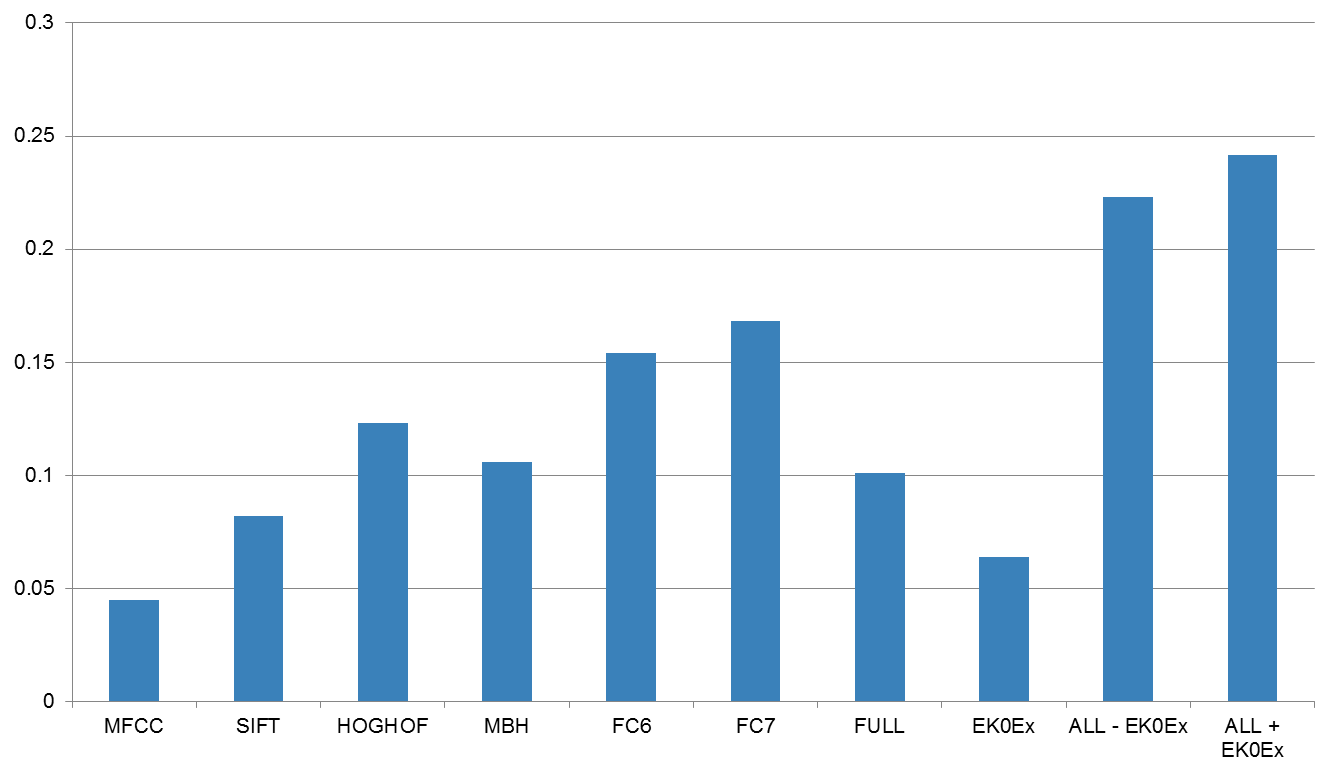
\includegraphics[width=1\textwidth]{feat_perf.png}
	\caption{Performance of each feature and the fused runs.}
	\label{fig_feat_perf}
\end{figure}

\section{Submitted Systems}

After evaluating the improvements on the KINDREDTEST dataset, we chose to submit the run that combining all available features for EK10 and EK100 settings. We also submit our EK0 system to the full evaluation.

\section{Result and Conclusion}

Results of our MED system on the full evaluation set is shown in Fig. \ref{result_team}. Performance is reported in terms of MAP. Comparing with other systems, we are ranked 6th out of 7 teams in the EK10 evaluation full and 6th out of 16 in the sub evaluation. 

We have learnt that top performance systems have incorporated a couple of semantic concept detectors including audio and visual concepts, which can be more helpful when number of training videos are limited. This is the reason for lower performance of our EK10 system.

On the other hand, our system performed better in EK100 the setting. For example, we got a better performance than the top team in this setting. This indicate that our low level features work well when the number of training videos is abundant. We also observed that our year-to-year improvement on EK10 is 72.5 \%, while this number is only 25.9\% for the EK100. This observation confirms the contributions of high level and deep learning features in case of event detection with few examplars.

\begin{figure}
	\centering
	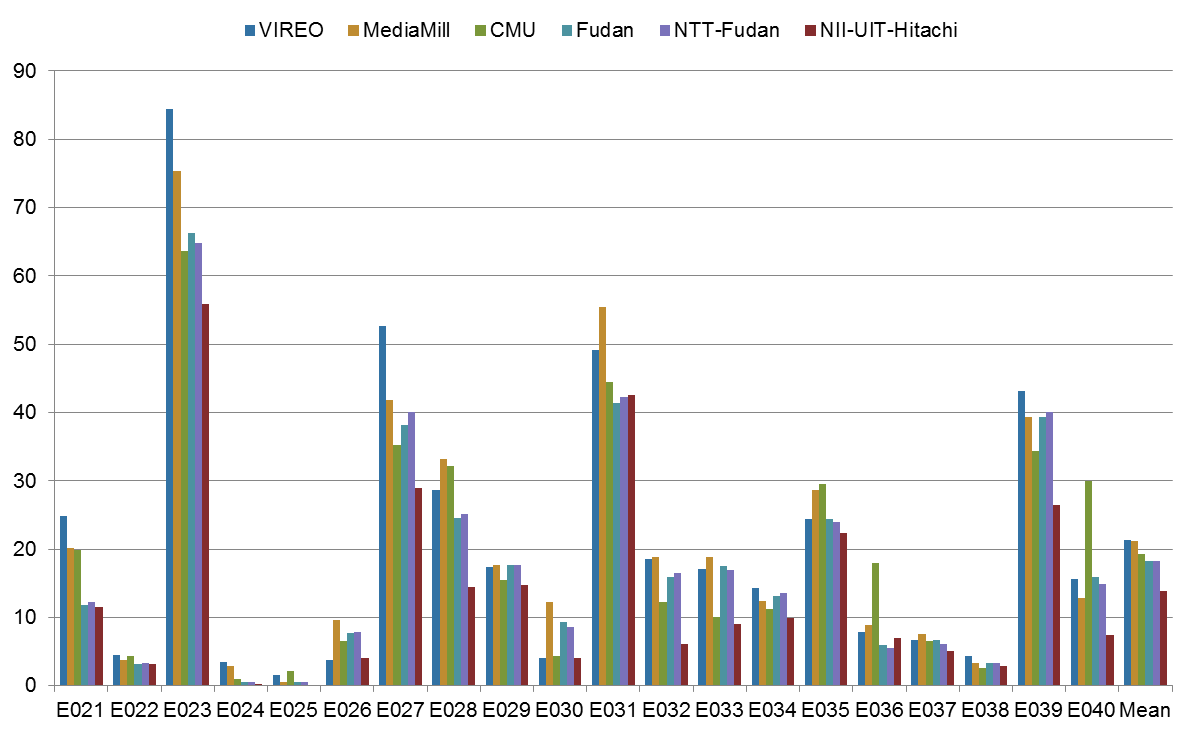
\includegraphics[width=1\textwidth]{result_team.png}
	\caption{Comparison of our performance with top systems in terms of MAP.}
	\label{result_team}
\end{figure}



